\chapter{Switchmode regulation}
\section{Theory and related work} \label{sec:literature_switchmode}

Switchmode regulators operate by rapidly switching an energy storage device on and off. The duty cycle and frequency of the switch sets how much charge is transferred to the load. This, in turn determines the output voltage of the regulator. These regulators can be used to step down(buck) or step up(boost) a given input voltage. The series storage device is usually either fully conducting or switched off, thus, the regulator tends to dissipate almost no power. This gives it quite a high efficiency. Due to the switching operation of the regulator, it produces a significant ripple voltage at its output. However, it is a much better choice if the input voltage is much higher than the output voltage \cite{regulators-main}.


\section{Design} \label{sec:design_switchmode}
\textbf{\textit{Design rationale}} \\
As explained in Section \ref{sec:rationale_system}, the switchmode regulator is used to give an intermediate voltage of that is then passed through the linear regulator designed in Section \ref{sec:design_linear}. This intermediate voltage is also used to power the charge pump scheme in Section \ref{sec:design_chargepump}. The intermediate voltage is chosen as \SI{9.5}{\volt} as shown to be sufficient in Section \ref{sec:design_chargepump}.

In terms of the design of the regulator, the device's datasheet provides a sufficient circuit that is implemented in the design \cite{LM2595}.The components listed below and shown in Figure \ref{fig:switchmode_circuit} are all chosen based of \cite{LM2595}, which provides the appropriate values to use for a wide reange of applications.

\begin{itemize}
    \item A low ESR capacitor is required at the input pin to prevent large voltage transients from appearing, and to provide the instantaneous current required each time the switch turns on.
    \item A feedforward capacitor adds lead compensation to the feedback loop and increases
    the phase margin for better loop stability.
    \item An output capacitor is required to filter the output and provide regulator loop stability. Low impedance/ ESR capacitors designed for switching regulator applications must be used.
    \item Buck(step-down) regulators require a diode to provide a return path for the inductor current when the switch turns off. Because of their very fast switching speed and low forward voltage drop, Schottky diodes provide the best performance.
    \item An inductor at the output is used to store energy such that current continuously flows, even when the regulator is "switched off". An inductor of $\SI{330}{\mu H}$ is suggested, but a smaller inductor is already provided. So, it is used as it will provide just as much or more continuous current.
    \item Resistors, R1 and R2 in Figure \ref{fig:switchmode_circuit}, are used to adjust the output voltage as shown in Equation \ref{eq:switchmode_output}.
    
\end{itemize}


\noindent\textbf{\textit{Design calculations}} \\
\textit{Feedback resistors/ Adjusting voltage output \cite{LM2595}:}
\begin{equation} \label{eq:switchmode_output}
    \begin{split}
        V_{out} &= (1+\frac{R_1}{R_2})V_{ref} \\
        R_1 &= R_2(\frac{V_{out}}{V_{ref}}-1) 
        = 1k(\frac{9.5}{1.23}-1) \\
        &=\SI{6.724}{\kilo\ohm}
    \end{split}
\end{equation}
A $\SI{10}{\kilo\ohm}$ variable resistor is placed at $R_1$ and set to give the required output voltage.


\noindent\textbf{\textit{Circuit diagram}}
\begin{figure}[h!]
 \centering
  	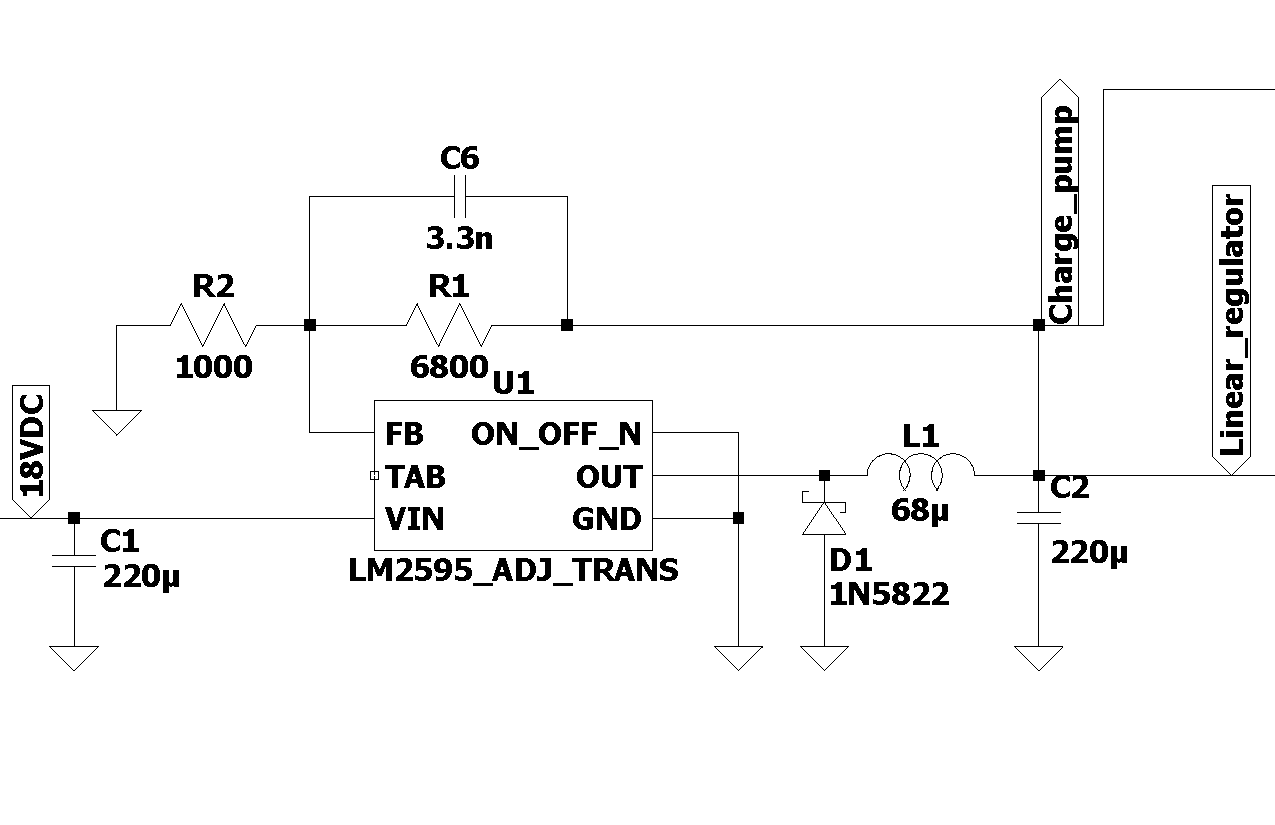
\includegraphics[width=0.55
  	\linewidth,clip,trim = 0cm 2.5cm 0cm 1cm]{./Figures/switchmode_circuit.pdf}
  	\caption{Switchmode regulator circuit.}
  	\label{fig:switchmode_circuit}
 \end{figure}


\section{Simulation} \label{sec:simulation_switchmode}
A plot of the LTSpice switchmode regulator simulation is given in Figure \ref{fig:switchmode_simulation}.
\begin{figure}[h] 
 \centering
  	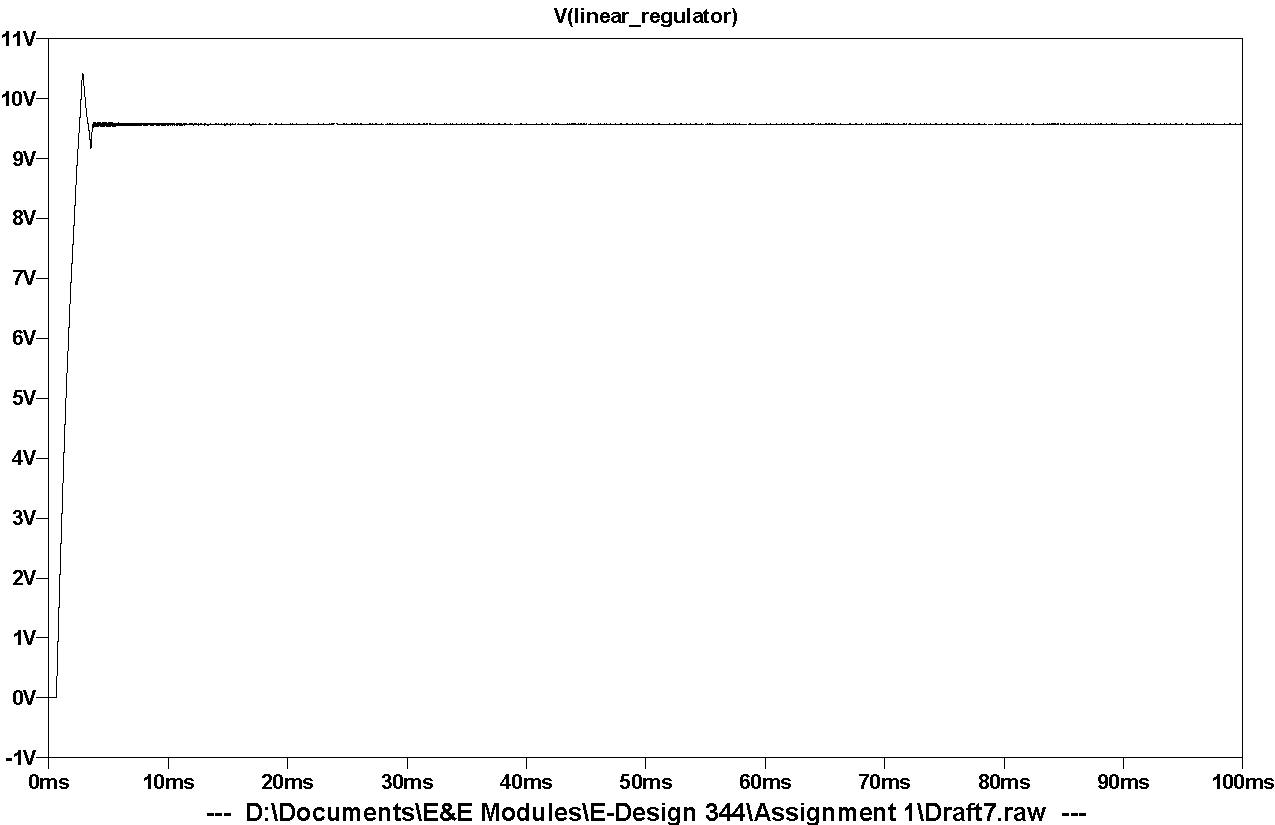
\includegraphics[width=0.7\linewidth]{./Figures/switchmode_simulate.pdf}
  	\caption{Simulated switchmode output.}
  	\label{fig:switchmode_simulation}
 \end{figure}
 
 
\section{Measurements} \label{sec:measurements_switchmode}
The measured output voltage from the switchmode is given in Figure \ref{fig:switchmode_measurement_box}.
\begin{figure}[h]
 \centering
        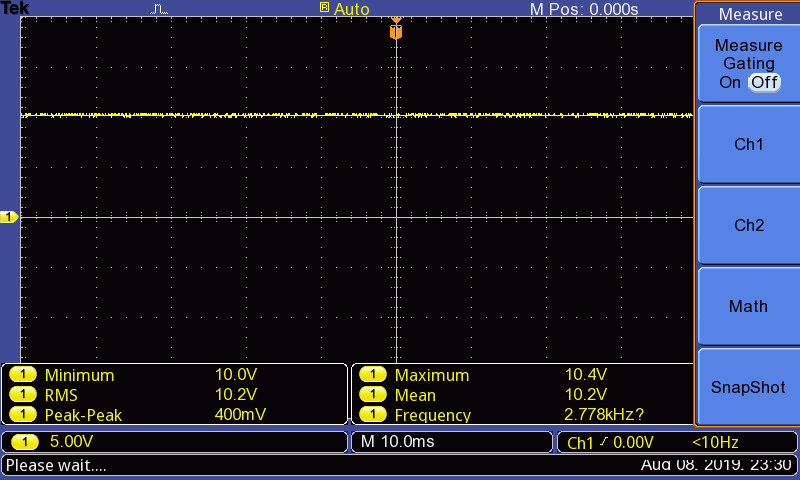
\includegraphics[width=0.6\linewidth,]{./Figures/switchmode_test}
        \caption{Switchmode output voltage}
\caption{Switchmode measured output}
\label{fig:switchmode_measurement_box}
\end{figure}







